\chapter{Standar LateX}

Pertama pahami dulu bagaimana bada isi file .tex yang akan kita kerjakan. Download atau lihat salah satu file \textit{LateX} yang akan kita kerjakan. Untuk mengisi \textit{LateX} kita harus mengisinya di dalam komponen yang merupakan \textit{tag} dengan pembuka \textit{begin} dan diakhiri dengan \textit{end}. Kemudian kenali bagian buku terdiri dari \textit{part}, \textit{chapter}, dan \textit{section}. \textit{Part} itu bisa kita andaikan \textit{bab}, \textit{subbab}, \textit{chapter}, dan \textit{section}, adalah bagian.

Kita bisa memisahkan isi dari \textit{LaTeX} dengan perintah input kemudian di dalam kurung kurawal letak file .tex yang akan kita masukkan kedalam file utama \textit{LaTeX} tersebut. \textit{LaTeX} merupakan program pengolahan kata atau sistem persiapan pembuatan dokumen untuk pengetikan sistem \textit{TeX}, yang dinamakan berdasarkan gaya penulisan-nya sebagai \textit{LaTeX}. Nama \textit{LaTeX} itu sendiri hanya mengacu pada bahasa penulisan yang digunakan pada sebuah dokumen, bukan pada editor yang digunakan untuk menulis dokumen tersebut. Untuk membuat dokumen dalam format \textit{LaTeX}, sebuah file berformat .tex harus dibuat menggunakan semacam \textit{text editor}. Walaupun, banyak \textit{text editor} yang dapat digunakan untuk membuat dokumen \textit{LaTeX}, beberapa \textit{text editor} sengaja dibuat khusus untuk menggunakan bahasa \textit{LaTeX}. Untuk panduan lebih lengkap silahkan kunjungi materi di \textbf{\textit{https://github.com/BukuInformatika
/keleketex}}

\section{Hello \textit{LaTeX}}
Ketikkan perintah dibawah ini pada \textit{text editor} anda :
		\begin{figure}[H]
		\centering
		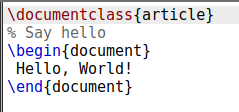
\includegraphics[width=1\textwidth]{figures/hello.png}
		\caption{Gambar hello latex}
		\end{figure}


